\documentclass[english]{article}

\usepackage{babel}
\usepackage{graphicx}
\usepackage{times}
\usepackage{pifont}
\usepackage[landscape,margin=2cm]{geometry}
\usepackage{eurosym}
\usepackage{fancyhdr}
\usepackage[hidelinks]{hyperref}
\usepackage{framed}
\usepackage[thinlines]{easytable}
\usepackage{enumitem}
\usepackage{float}

\pagestyle{fancy}
\fancyhf{}


%HEADER
%**************************************************************************************
\pagestyle{fancy}
\fancyhf{}
%**************************************************************************************
\lhead{Space Monitor}		 	 
\rhead{Final report} 
\lfoot{Computer Service Management}
\cfoot{\thepage}
\rfoot{Alexey Tukalo}
%**************************************************************************************

\date{}
\setlength\parindent{0pt}

\begin{document}

\title{\vspace{2in}Space Monitor}

\nopagebreak
\maketitle


\vspace{2.5in}

\author{
\begin{flushright}
Alexey Tukalo,\\
Computer Service Management,\\
Institute of technology Tralee
\end{flushright}
}

\date{\today}
\thispagestyle{empty}

\newpage
\setcounter{page}{1}
\setcounter{tocdepth}{2}
\tableofcontents

\newpage
\section{Scope Statement}
\begin{framed}
\textbf{Project Title:  Space monitor } \\
\textbf{Date: \today}
\textbf{Prepared by: April 27, 2015 }
\end{framed}
\begin{framed}
  \textbf{Project Justification:} \\
  The aim is to develop project with complex network architecture, the project should contain microcontroller which communicates with server over internet and the webpage which demonstrate the sensors work in visual way. The project have to follow philosophy of internet of things.
  \end{framed}
  \begin{framed}
   \textbf{Product Characteristics and Requirements:}
\begin{enumerate}
  \item The microcontroller have to:
  \begin{enumerate}
  \item transmit data over internet to the server
  \item read data from Ultrosonic sensor 
	\end{enumerate}
  \item The server have to:
    \begin{enumerate}
  \item received data from microcontroller
  \item keep data in the database
  \item provide RESTfull API for webpage
  \item be based on IBM BlueMix
	\end{enumerate}
  \item The webpage have to:
    \begin{enumerate}
  \item be implement fluid-design 
  \item contain:
  \begin{enumerate}
  \item legend
  \item two donut chart
  \item bar chart
  \item plot
	\end{enumerate}
  \item receive data from RESTfull API
	\end{enumerate}
\end{enumerate}
  \end{framed}
  \begin{framed}
  \textbf{Summary of Project Deliverables}\\
  
 \textbf{Project management-related deliverables: }the following documentation and any other documents required to manage the project.
 \begin{enumerate}
  \item  Scope statement
  \item WBS
  \item Network diagram and critical path
  \item Risk register and probability impact matrix
  \item Communication plan
  \item Cost baseline
  \item Team contract
  \item Project completion report
	\end{enumerate}


 \textbf{Product-related deliverables:}
  \begin{enumerate}
  \item A project meeting the agreed specification
  \item A design document detailing the project architecture
  \item All software code
  \item Final presentation
	\end{enumerate}


\textbf{Non Project Deliverables}
  \begin{enumerate}
  \item No guarantee of increased revenue for the project
  \item The ongoing site maintenance following the completion of the project
  \item The website hosting and hosting contract
  \item The website launch
	\end{enumerate}
  \end{framed}
  \begin{framed}
  \textbf{Project Success Criteria:} \\
   \begin{enumerate}
  \item The project will be completion within 3 months.
  \item All HTML and CSS to validate to W3C standards.
  \item The project will be fully functional
  \item The product will follow Product Characteristics and Requirements
	\end{enumerate}
  \end{framed}
  \begin{framed}
\textbf{Assumptions:} \\
 The project team will consist of a Sponsor(University) and Project Manager/Programmer(Alexey Tukalo) and Programmers(Gaëtan M., Florian Henriet).
\end{framed}

\section{Risk Register}

\begin{tabular}{|p{0.5cm}|p{2.5cm}|p{4cm}|p{1.5cm}|p{1.5cm}|p{1.5cm}|p{1.5cm}|p{1.5cm}|p{6cm}|}
  \hline  
No & Risk & Description & Rank & Affected Areas & Probability & Impact & Owner & Potential Responses \\
  \hline  
1 &
Loss of funding &
Loss of funding for hardware & 
Medium & 
Scope, Schedule & 
Low & 
Low & 
U & 
Use hardware already available at University \\
  \hline  
  2 &
Teammate illness &
Teammate is sick and not able to work  & 
Medium & 
Schedule & 
Medium & 
Medium & 
T & 
Reallocate tasks of the sick teammate between other developers \\
  \hline  
    3 &
Hardware problems &
Hardware problems during development & 
High & 
Scope, Schedule, Cost & 
High & 
Low & 
T & 
Troubleshoot the device, repair or buy new\\
  \hline  
      4 &
BlueMix failure &
BlueMix Cloud is unavailable for some reason  & 
High & 
Scope, Quality, Schedule, Cost & 
Low & 
High & 
B & 
Move server to other cloud or build own server\\
  \hline 
 5 &
Aliens attack &
Civilisation from far space captured control under the Earth & 
High & 
Scope, Quality, Schedule, Cost & 
Low & 
High & 
A & 
Join partisan detachments resistance, stop developing, the product is useless in case of Galactic war \\
  \hline 
  
\end{tabular}

\begin{tabular}{ l l}
\\
Prepared by: Alexey Tukalo & Date: \today \\

\end{tabular}\\\\
Owners:\\
\begin{tabular}{l l l}
U & University & Project sponsor\\
T & Team & Project team\\
B & IBM BlueMix & Supplier\\
A & Aliens & Aliens from far space\\
\end{tabular}
\newpage


\section{Communication Plan }

\begin{tabular}{l l}
Date: \today  & Prepared by: Alexey Tukalo\\
\end{tabular}\\
\begin{tabular}{|p{3cm}|p{5cm}|p{3cm}|p{4cm}|p{1.5cm}|p{5cm}|}
\hline
Method & Purpose & Responsibility & Audience & Frequency & Deliverable\\
\hline
Meeting & 
Get project requirements, ask question about unclear statements &
Supervisor &
Supervisor, Dev Team &
Once off &
List of the project requirements \\
\hline 
Meeting(brainstorm) & 
Create the idea of the project in accordance with the specification &
Project Manager &
Dev Team &
Once off &
Concept of the project \\
\hline 
Meeting & 
Discuss the project concept with supervisor, get advices and permission &
Project Manager &
Supervisor, Dev Team &
Once off &
Permission for a future development of the concept\\
\hline 
Meeting & 
Reconcile the scope statement of the project with supervisor &
Project Manager &
Supervisor, Dev Team &
Once off &
Permission to start actual development of the system\\
\hline 
Meeting (brainstorm) & 
Develop an architecture of the system &
Project Manager &
Dev Team &
Once off &
Plan of the system architecture\\
\hline 
Meeting (brainstorm) & 
Identify the technological implementation of the architecture &
Project Manager &
Dev Team &
Once off &
Technical plan of the project\\
\hline 
Meeting (brainstorm) & 
Identify the details of data transmission in the system &
Project Manager &
Dev Team &
Once off &
Format of the JSON object\\
\hline 
Meeting & 
Spread the project into independent parts with equal scope and spread the roles between developers &
Project Manager &
Dev Team &
Once off &
Reconcile roles in the Dev Team\\
\hline 
Meeting & 
Set deadlines, identify steps of the project development &
Project Manager &
Dev Team &
Once off &
Plan of the development (Gantt chart)\\
\hline 
Meeting & 
Create a list of hardware for project implementation &
Project Manager &
Dev Team &
Once off &
Resource list\\
\hline 
Meeting & 
Demonstrate results to the supervisor &
Project Manager &
Supervisor, Dev Team &
Once off &
Feedback from the supervisor\\
\hline 
Presentation & 
Present project in University &
Project Manager &
Supervisor, Dev Team, other students and teacher &
Once off &
Feedback from the focus group \\
\hline 
Skype conversation & 
Discuss particular development process and problems with teammates &
All team member &
Dev Team &
any time &
Exchange opinions with other teammate about particular problems, share results \\
\hline 
Meeting & 
Discuss particular development process with supervisor &
Project Manager &
Supervisor, Dev Team &
Weekly &
Progress reports\\
\hline 
\end{tabular}
\\\\\\
Documents: 
\\\\
List of the project requirements: list of requirements to the project from supervisor
\\\\
Concept of the project: detailed an explanation of the general idea behind the project.
\\\\
Plan of the system architecture: an abstract plan of the project's software and hardware implementations and a network diagram.
\\\\
Technical plan of the project: detailed plan of the project's software and hardware implementation.
\\\\
Format of the JSON object: example of the JSON object used to transmit data between components of the system.
\\\\
Plan of the development: Gantt chart with steps of development, responsible people and deadlines.
\\\\
Resource list: list of hardware resources required for realisation of the project prototype.
\\\\
Progress report: the Project Manager will maintain a record of project work and will record decisions made, along with budgetary and timeline monitoring.
\section{Work time Exceptions}
\vspace{1cm}
\begin{center}
\begin{large}
Florian
\end{large}\\
\begin{tabular}{|l|p{5cm}|c|c|}
\hline
1 & Business trip & 01.4.2015 & 07.4.2015 \\
\hline
2 & Fishing & 18.4.2015 & 19.4.2015\\
\hline
\end{tabular}\\
\vspace{1cm}
\begin{large}
Geaten
\end{large}\\
\begin{tabular}{|l|p{5cm}|c|c|}
\hline
1 & Attending conference & 11.4.2015 & 13.4.2015 \\
\hline
\end{tabular}\\
\vspace{1cm}
\begin{large}
Alex
\end{large}\\
\begin{tabular}{|l|p{5cm}|c|c|}
\hline
1 & Stolen by aliens & 24.4.2015 & 27.4.2015 \\
\hline
2 & Attending conference & 1.5.2015 & 3.5.2015 \\
\hline
\end{tabular}

\end{center}
\section{Probability/Impact Matrix}
Probability\\
\begin{TAB}(b,6cm,3cm){c|c|c|c|}{|c|c|c|c}
high & Hardware problems & - & -\\

medium & - & Teammate illness  & - \\

low & Loss of funding & -  & BlueMix failure,
							 Aliens attack\\

- & low & medium & high \\
\end{TAB}
\begin{center}Impact\end{center}

\section{WBS}
\begin{enumerate}
\item Idea creation
	\begin{enumerate}[label*=\arabic*]
	\item Get requirements
	\item Create concept (brainstorm)
	\item Reconcile the project the concept with supervisor
	\item Reconcile scope statement
	\item Prepare abstract
	\item Consept is ready
	\end{enumerate}
\item Planning
	\begin{enumerate}[label*=\arabic*]
	\item Develop the architecture of system
	\item Identify the technologies
	\item Identify the details of data transmission
	\item Separate roles between team members
	\item Set deadlines for development
	\item Create resource list
	\item Create reasource list
	\item Order hardware
	\item Plan is ready
	\end{enumerate}
\item Development 
	\begin{enumerate}[label*=\arabic*]
	\item Webpage
		\begin{enumerate}[label*=\arabic*]
		\item Create design
		\item Parse data
		\item Create layout
		\item Create donut charts
		\item Create bar chart
		\item Create plot
		\item Add legend
		\item Add tooltips
		\end{enumerate}
	\item Server
		\begin{enumerate}[label*=\arabic*]
		\item Install MongoDB
		\item Set connection to IoT
		\item Create server logic at Node-red
		\item Turn on API for Web Page
		\end{enumerate}
	\item Sensor
		\begin{enumerate}[label*=\arabic*]
		\item Install driver and set IDE
		\item Stick together hardware
		\item Read data from the sensor
		\item Send data to the server
		\end{enumerate}
	\item Integration of the system
		\begin{enumerate}[label*=\arabic*]
		\item Test system together
		\item Fix problems
		\item System is integrated
		\end{enumerate}
	\end{enumerate}
\item Testing
	\begin{enumerate}[label*=\arabic*]
	\item Test the system in real life case
	\item Confirm HTML and CSS code validate to W3C standards
	\item Test visualisation on different browsers and screen sizes
	\item Fix problems
	\item Show result to supervisor and get feedback
	\item Make final editions in according with supervisor's feedback
	\item Testing is pasted
	\end{enumerate}
\item Closing 
	\begin{enumerate}[label*=\arabic*]
	\item Prepare final report
	\item Final presentation
	\item Project is ready
	\end{enumerate}
\end{enumerate}
\section{Milestones}
\begin{tabular}{p{5cm}|p{5cm}}
Start & 3/2/15 8:00 AM
 \\\\
Concept is ready & 3/30/15 9:00 AM
\\\\
Plan is ready & 4/6/15 2:00 PM
\\\\
System is integrated & 5/11/15 2:00 PM
\\\\
Testing is pasted & 5/20/15 4:00 PM
\\\\
Project is ready & 5/25/15 2:00 PM


\end{tabular}
\newpage
\section{Appendix}
\subsection{Milestones}
\begin{figure}[H]
\centerline{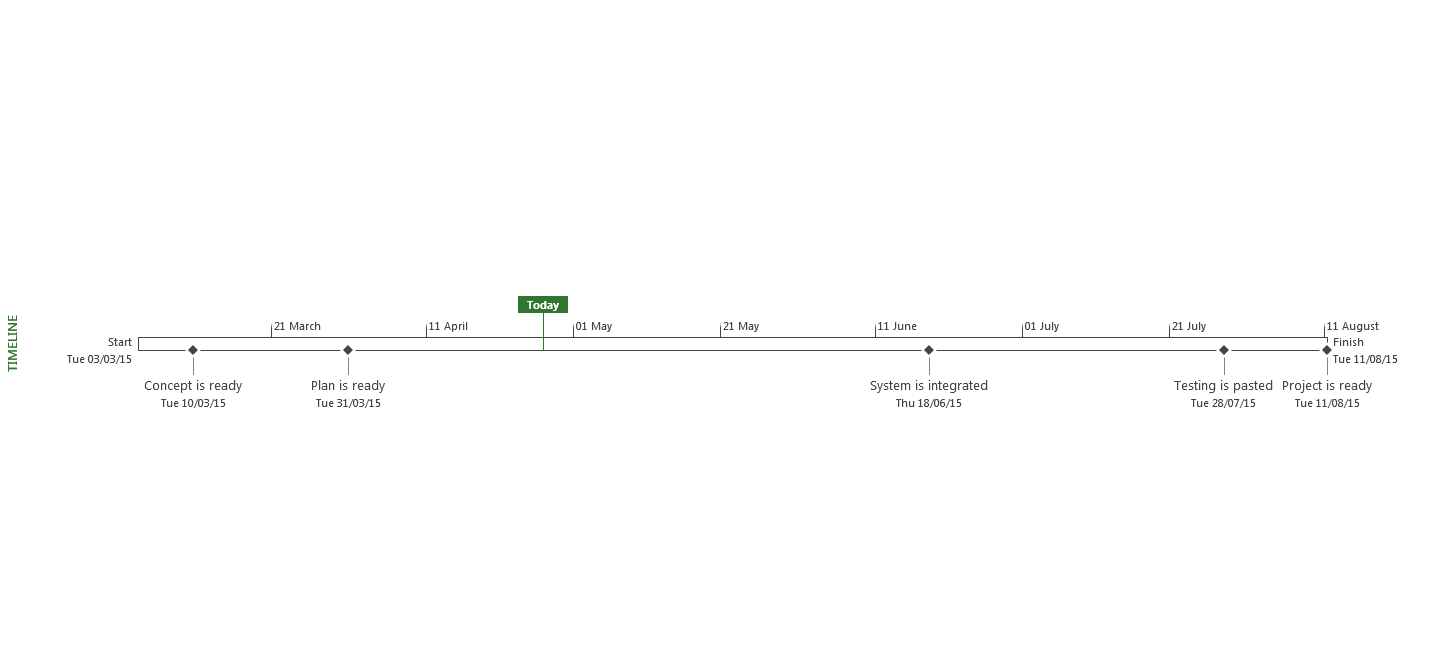
\includegraphics[scale=0.6]{FR/timeline}}
\end{figure}
\newpage
\subsection{Cost overview}
\begin{figure}[h]
\centerline{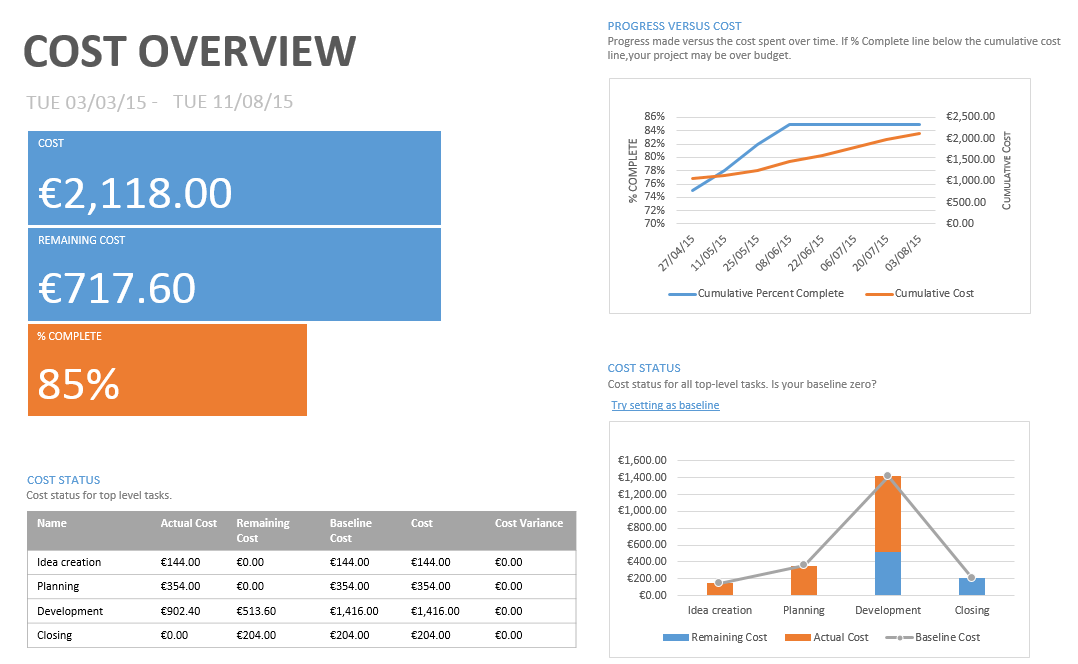
\includegraphics[scale=0.77]{FR/costs}}
\end{figure}
\newpage
\subsection{Earned Value over time}
\begin{figure}[H]
\centerline{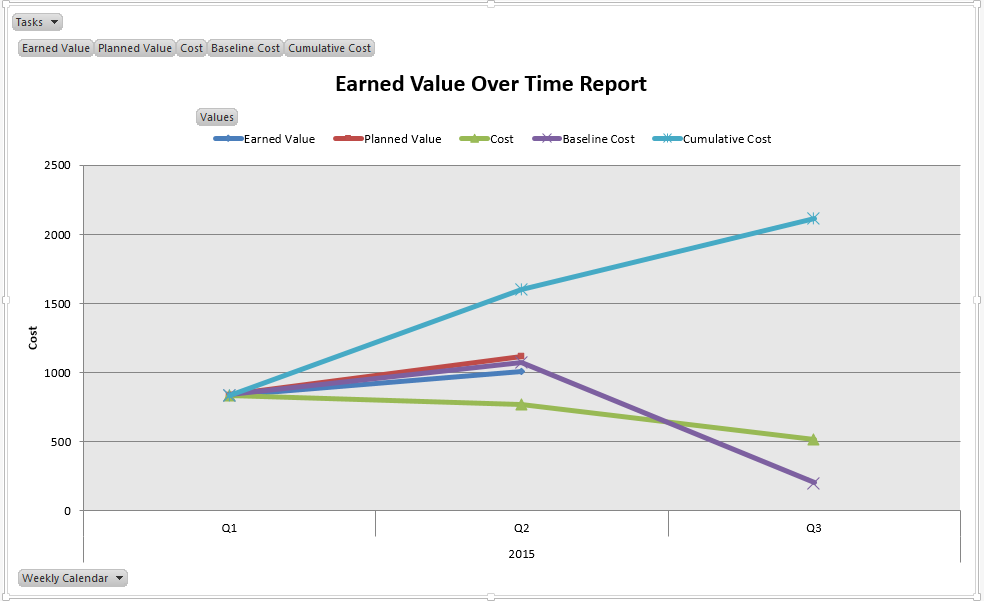
\includegraphics[scale=0.8]{FR/ev}}
\end{figure}
\subsection{Milestones Report}
\begin{figure}[H]
\centerline{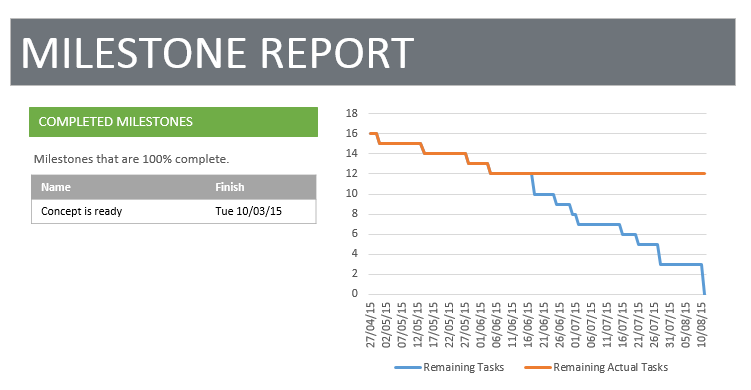
\includegraphics[scale=1]{FR/ml}}
\end{figure}
\newpage
\subsection{Resource overview}
\begin{figure}[H]
\centerline{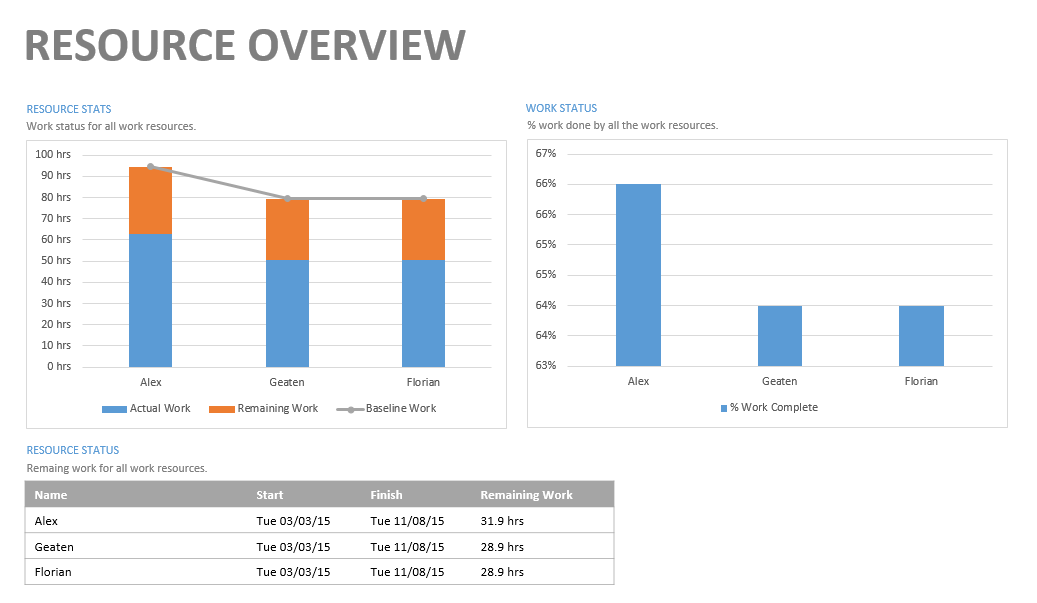
\includegraphics[scale=0.8]{FR/resoursec}}
\end{figure}
\subsection{Delay in project schedule}
\begin{figure}[H]
\centerline{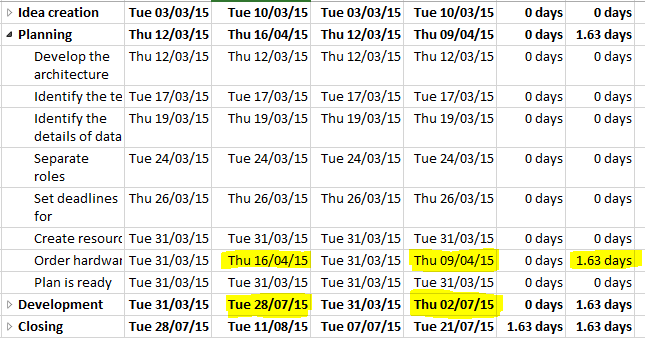
\includegraphics[scale=1]{FR/slack}}
\end{figure}
\subsection{Top level tasks}
\begin{figure}[H]
\centerline{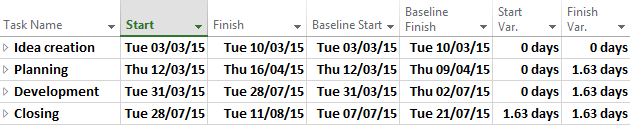
\includegraphics[scale=1]{FR/bt}}
\end{figure}
\subsection{Project overview}
\vspace{1in}
\begin{figure}[H]
\centerline{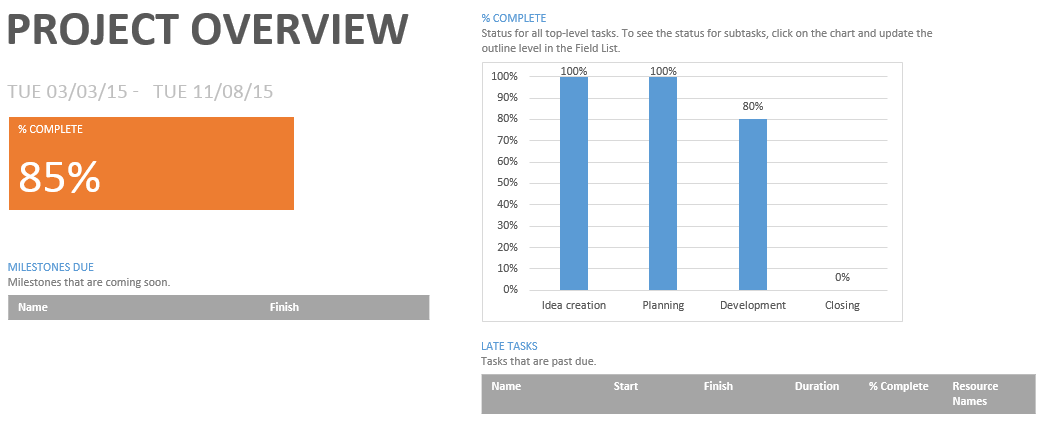
\includegraphics[scale=0.8]{FR/pj}}
\end{figure}
\subsection{Resource cost overview}
\begin{figure}[H]
\centerline{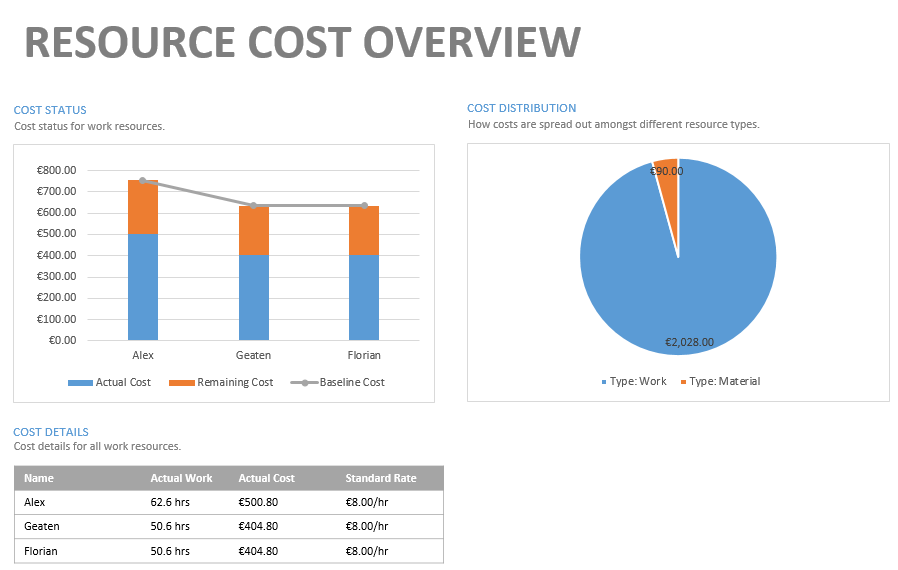
\includegraphics[scale=1]{FR/rco}}
\end{figure}
\subsection{Task cost overview}
\begin{figure}[H]
\centerline{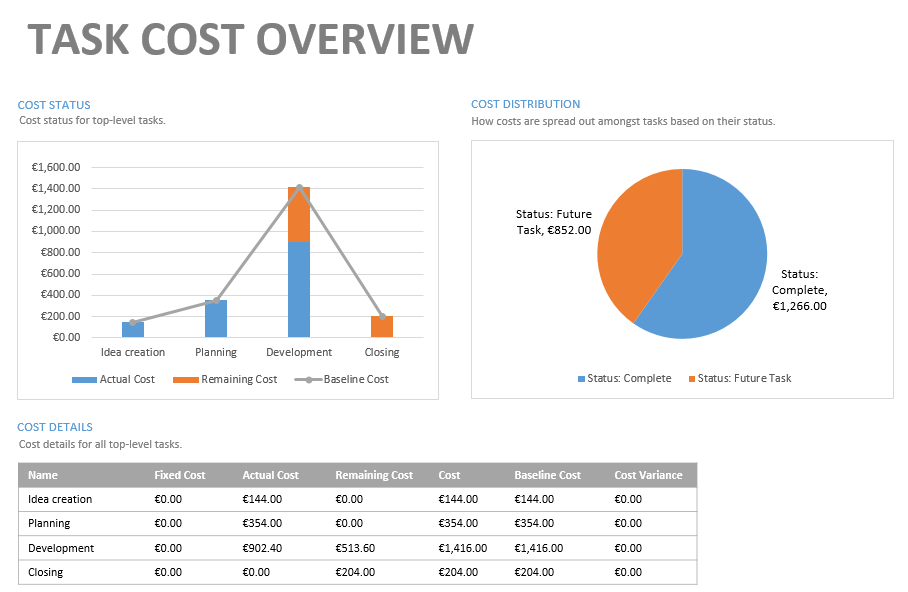
\includegraphics[scale=1]{FR/tco}}
\end{figure}
\subsection{Work Overview}
\begin{figure}[H]
\centerline{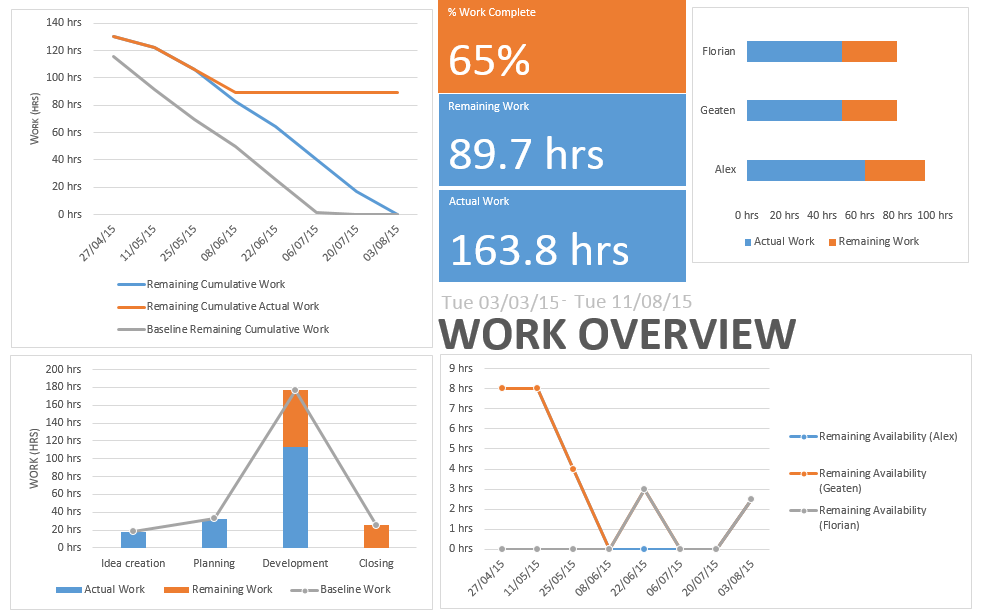
\includegraphics[scale=0.8]{FR/wo}}
\end{figure}


\end{document}
